\section{Test}


\begin{figure}[h]
\centering
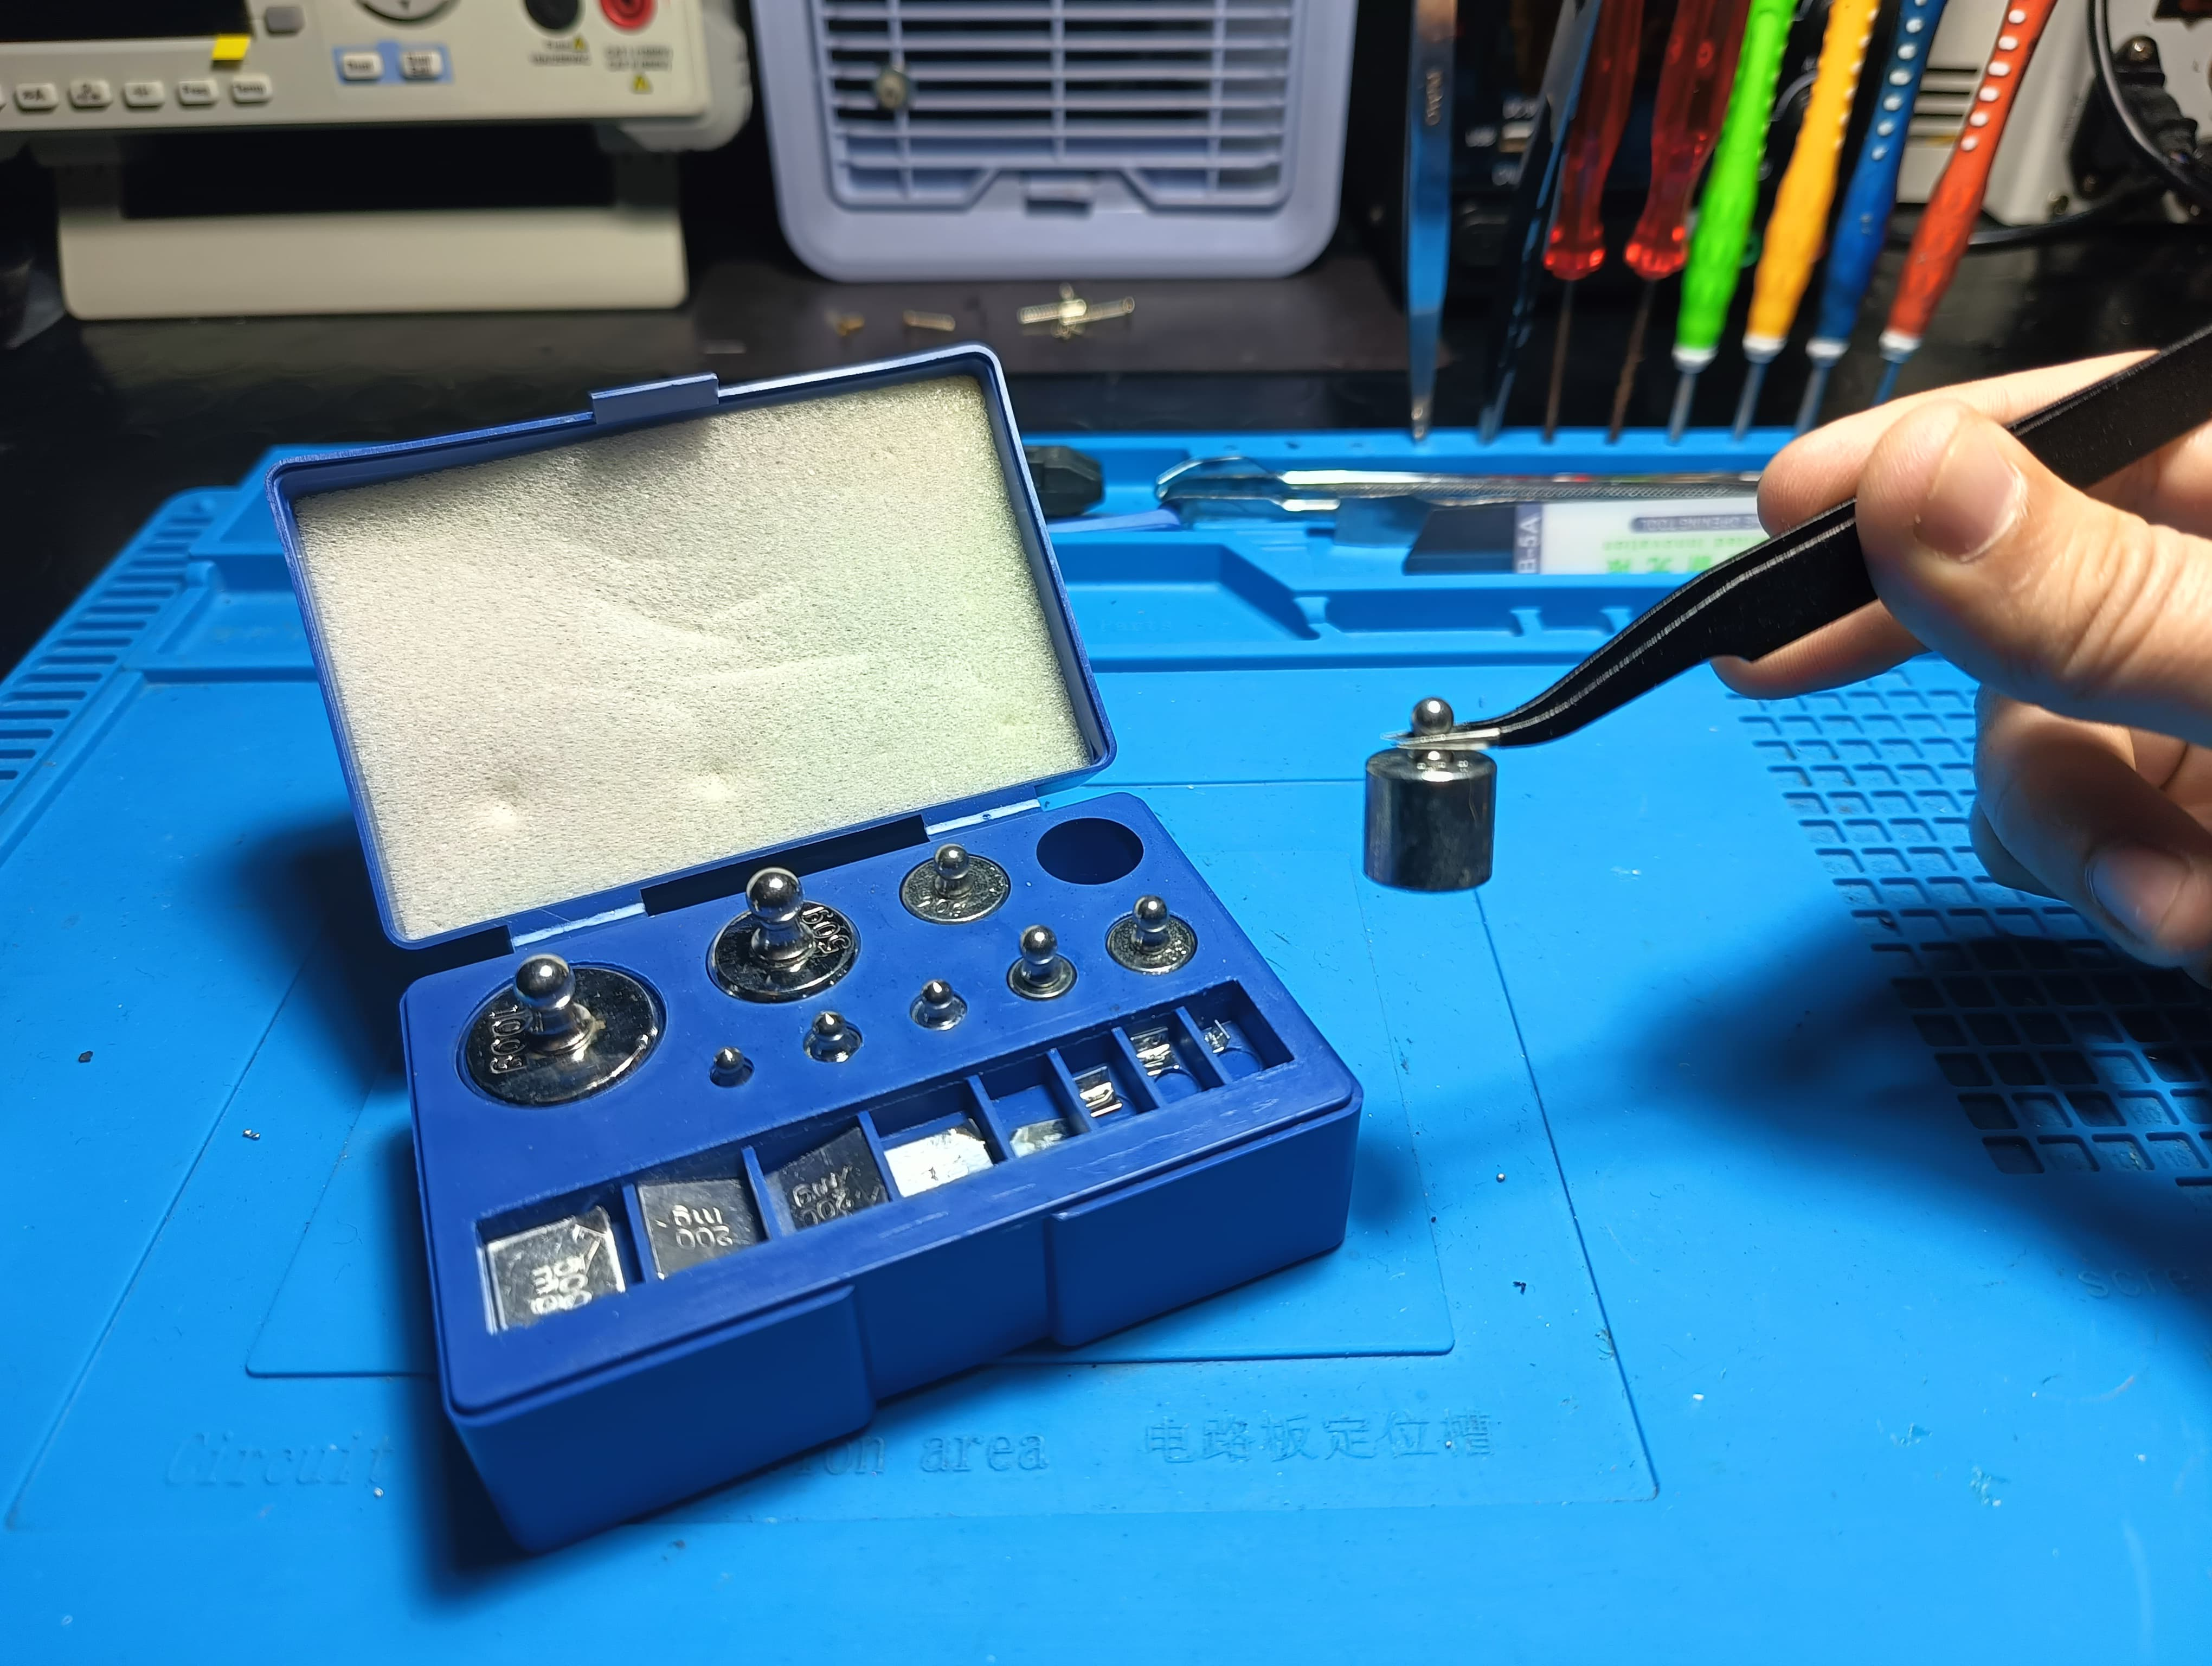
\includegraphics[width=\textwidth]{medias/parts/sample_weights.jpeg}
\caption{Test with sample weights}
\end{figure}
\clearpage

\section{Calibration}

We are trying to calibrate this scale using an iterative method to find the calibration factor and the offset that minimize the error between the actual weight and the measured weight. To do this, you can use the following formula:

\[
\text{Actual weight} = \text{Measured weight} \times \text{Cf} + \text{Offset}
\]
\noindent
To calculate the error, we can use the following formula:

\[
\text{Error} = \sum_{i=1}^{n} (\text{Actual weight}_i - \text{Measured weight}_i \times \text{Cf} - \text{Offset})^2
\]
\noindent
Where $n$ is the number of weights used in each iteration.\\
To find the Cf and the Offset that minimize the error, we use the gradient method, which consists of changing the values of Cf and Offset according to the derivative of the error with respect to them, using the following formulas:

\[
\text{New Cf} = \text{Cf} - \alpha \frac{\partial \text{Error}}{\partial \text{Cf}}
\]

\[
\text{New Offset} = \text{Offset} - \alpha \frac{\partial \text{Error}}{\partial \text{Offset}}
\]
\noindent
Where $\alpha$ (also called learning rate) is a parameter that controls the convergence rate of the method. The value of $\alpha$ is chosen so that it is small enough to avoid swings, but large enough to reach the minimum in a few iterations.\\
To calculate the partial derivatives of the error, we need to use the following formulas:

\[
\frac{\partial \text{Error}}{\partial \text{Cf}} = -2 \sum_{i=1}^{n} (\text{Actual weight}_i - \text{Measured weight}_i \times \text{Cf} - \text{Offset}) \times \text{Measured weight}_i
\]

\[
\frac{\partial \text{Error}}{\partial \text{Offset}} = -2 \sum_{i=1}^{n} (\text{Actual weight}_i - \text{Measured weight}_i \times \text{Cf} - \text{Offset})
\]
\noindent
In reality, for the calculation of Cf and offset, we are using an empirical formula, that is, adding the error with a certain weight to the previously calculated values:

\[
\text{New Cf} = \text{Cf} - \beta \times \text{Error}
\]

\[
\text{New Offset} = \text{Offset} - \beta \times \text{Error}
\]
\noindent
Where $\beta$ is a kind of learning rate, suitably tuned to get progressively better results.

\subsection{Procedure}

Wanting to go through the entire calibration process in depth:

\begin{itemize}
\item We prepared 6 iterations, with gradually smaller ranges, using sample weights:

\begin{tabular}{|c|c|c|}
\hline
\textbf{Iteration} & \textbf{Range} & \textbf{Increment} \\
\hline
0 & 0g-100g & 10g \\
1 & 0g-50g & 5g \\
2 & 0g-5.5g & 0.5g \\
3 & 0g-2g & 0.2g \\
4 & 0g-0.5g & 0.05g \\
5 & 0g-0.2g & 0.02g \\
\hline
\end{tabular}

\item We placed each weight for 5 points of the plate (center and the four corners)

\item Using MATLAB, we used a regression algorithm to fit the collected data The slope of the regression line represents the calibration factor and the intercept represents the offset, using the Euclidean norm (norm 2) to evaluate the error.

\item Last we used the data calculated by calibration, using it when compiling the microcontroller program.
\end{itemize}

\subsection{MATLAB pseudocode}

\begin{verbatim}
clear the workspace and the screen
reset the serial devices

set the number of objects
create a matrix of zeros to store the measures
create two vectors of zeros to store the weights

create and open a serial connection with the scale

wait until the scale is ready

for each object
    print a new line
    for each position from 1 to 5
        if the position is 1 (middle)
            ask the user to enter the known weight and place the object in the middle
            validate the input
            store the known weight in the vector x
            print a new line
        else if the position is 2 (bottom left)
            ask the user to place the object in the bottom left
        else if the position is 3 (top left)
            ask the user to place the object in the top left
        else if the position is 4 (top right)
            ask the user to place the object in the top right
        else if the position is 5 (bottom right)
            ask the user to place the object in the bottom right
        send a signal to the scale
        read the measured value from the scale
        store the measured value in the matrix measures
        print the measured value
    end for
end for

close and delete the serial connection
reset the serial devices

for each object
    calculate the average of the measures for that object
    store the average in the vector y
end for

create a table with the vectors x and y
save the table as a text file
save the table as a csv file

find the coefficients of the best fitting line for the data
the slope is the calibration factor
the intercept is the offset
evaluate the line at the known weights
compute the error vector
compute the error norm
print the error

create and clear a figure
plot the data as green circles
plot the line as a solid line
\end{verbatim}

\subsection{Stop condition}

For calibration, we have to find the right compromise to make the regression line fit, considering that we have to use a smaller and smaller range of weights until we arrive at a measurement that is not fouled by noise in such a way that the behavior of the scale is no longer linear. We found that up to the third iteration we still have linear behavior, with a larger error than in the second iteration, as the distance between the points and the line increases. Using a smaller range would mean that the measurements are greatly affected by noise, increasing the error as we try to fit a line into a nonlinear set of points.

\subsubsection{Iteration 0}

\begin{figure}[ht]
\centering
\begin{minipage}{.6\textwidth} % 60% della larghezza del testo
  \centering
  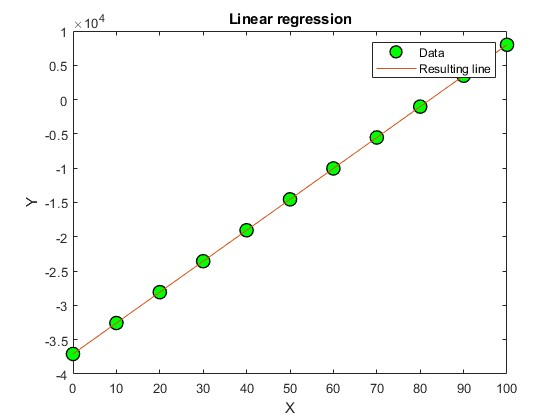
\includegraphics[width=.9\linewidth]{medias/test/calibration/figure_0.jpg}
  \captionof{figure}{Regression}
  \label{fig:test1}
\end{minipage}%
\begin{minipage}{.4\textwidth} % 40% della larghezza del testo
  \centering
  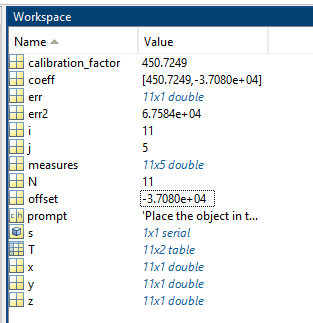
\includegraphics[width=.9\linewidth]{medias/test/calibration/workspace_0.png}
  \captionof{figure}{Workspace}
  \label{fig:test2}
\end{minipage}
\end{figure}


\subsubsection{Iteration 1}

\begin{figure}[H]
\centering
\begin{minipage}{.6\textwidth} % 60% della larghezza del testo
  \centering
  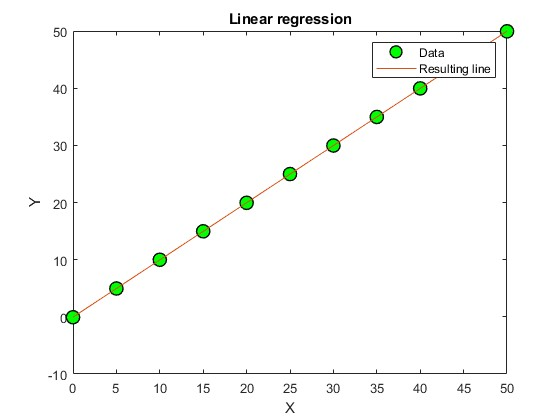
\includegraphics[width=.9\linewidth]{medias/test/calibration/figure_1.jpg}
  \captionof{figure}{Regression}
  \label{fig:test3}
\end{minipage}%
\begin{minipage}{.4\textwidth} % 40% della larghezza del testo
  \centering
  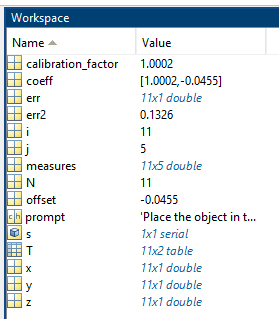
\includegraphics[width=.9\linewidth]{medias/test/calibration/workspace_1.png}
  \captionof{figure}{Workspace}
  \label{fig:test4}
\end{minipage}
\end{figure}

\subsubsection{Iteration 2}

\begin{figure}[ht]
\centering
\begin{minipage}{.6\textwidth} % 60% della larghezza del testo
  \centering
  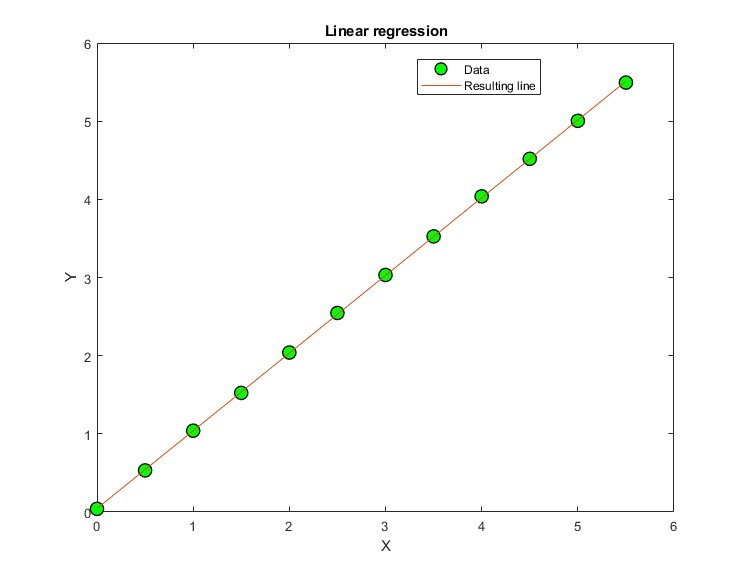
\includegraphics[width=.9\linewidth]{medias/test/calibration/figure_2.jpg}
  \captionof{figure}{Regression}
  \label{fig:test5}
\end{minipage}%
\begin{minipage}{.4\textwidth} % 40% della larghezza del testo
  \centering
  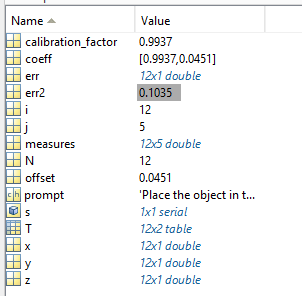
\includegraphics[width=.9\linewidth]{medias/test/calibration/workspace_2.png}
  \captionof{figure}{Workspace}
  \label{fig:test6}
\end{minipage}
\end{figure}

\clearpage

\subsubsection{Iteration 3}

\begin{figure}[ht]
\centering
\begin{minipage}{.6\textwidth} % 60% della larghezza del testo
  \centering
  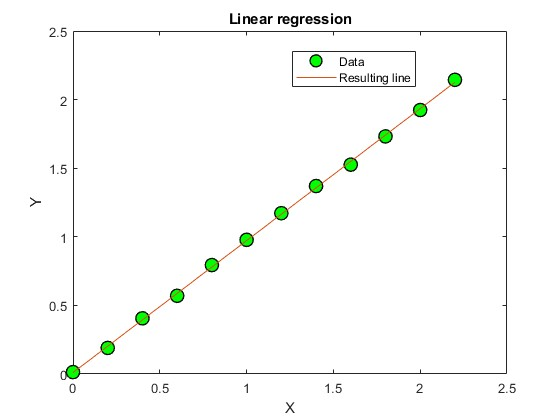
\includegraphics[width=.9\linewidth]{medias/test/calibration/figure_3.jpg}
  \captionof{figure}{Regression}
  \label{fig:test7}
\end{minipage}%
\begin{minipage}{.4\textwidth} % 40% della larghezza del testo
  \centering
  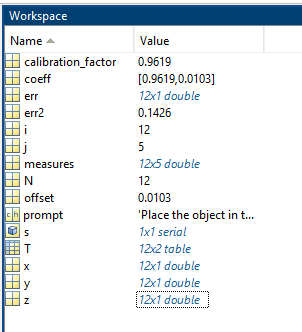
\includegraphics[width=.9\linewidth]{medias/test/calibration/workspace_3.png}
  \captionof{figure}{Workspace}
  \label{fig:test8}
\end{minipage}
\end{figure}

\subsubsection{Iteration 4}

\begin{figure}[ht]
\centering
\begin{minipage}{.6\textwidth} % 60% della larghezza del testo
  \centering
  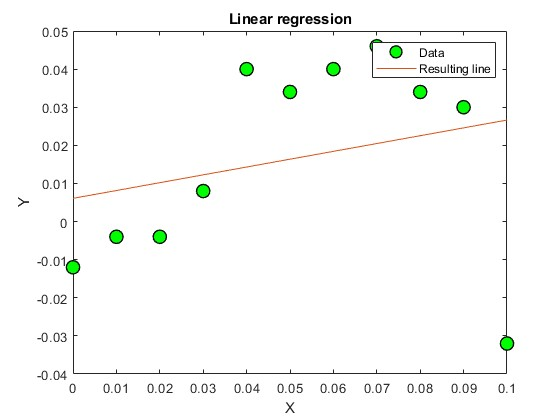
\includegraphics[width=.9\linewidth]{medias/test/calibration/figure_4.jpg}
  \captionof{figure}{Regression}
  \label{fig:test9}
\end{minipage}%
\begin{minipage}{.4\textwidth} % 40% della larghezza del testo
  \centering
  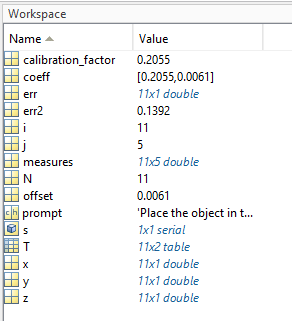
\includegraphics[width=.9\linewidth]{medias/test/calibration/workspace_4.png}
  \captionof{figure}{Workspace}
  \label{fig:test10}
\end{minipage}
\end{figure}


\begin{quote}
In this graph, it can be seen that variations on the order of hundredths of a gram are not appreciable, as the noise mat is of the same order of magnitude, so it makes the regression results much worse when calculating Cf and offset. Taken this into account, the 5th iteration wouldn't have much meaning.
\end{quote}

\clearpage

\subsection{Results}

In truth, already the first iteration returns us a plausible value of Cf, but this can be further improved. The same applies to the offset as well. The best result was achieved at the second iteration, when the range of values is small, but the variations between weights are still appreciable. In addition, we noticed that when the variation falls below 0.5 grams it starts to feel particularly noisy, so the measurements are more degraded. This, counterintuitively gives worse results, and as can be seen from the third iteration, will give a larger error and worse Cf and offset values than those calculated before.

\section{Noise}

The purpose of the noise test was to evaluate the accuracy and stability of the balance without any weights on it. We expected the balance to output zero or very small values when no weight was applied. However, due to various sources of noise, such as electrical interference, mechanical vibrations, or environmental factors, the balance might output some non-zero values.
\\
To perform the noise test, we collected 100 samples from the balance using Matlab, receiving a floating-point number representing the weight in grams from the scale. We repeated this process 100 times and stored the values in a vector n. We also saved the data in a table T and exported it to a text file and a csv file.
\\
We then analyzed the data using Matlab. We calculated the mean and the standard deviation of the vector n to get an estimate of the average noise level and the noise variance. We also plotted the frequency spectrum of the vector n using the discrete Fourier transform (DFT) to identify any dominant frequency components in the noise.
\\
The results of the noise test are shown below. The mean of the vector n is 0.12 g and the standard deviation is 0.07 g. This means that the balance has a very low noise level and a high accuracy. The frequency spectrum of the vector n shows that the noise is mostly random and does not have any significant peaks. This means that the balance is stable and does not suffer from any periodic disturbances.

\subsection{MATLAB pseudocode}

\begin{verbatim}
clear the workspace and the screen
reset the serial devices

Set N to 100
Create a vector of N elements, initialized to zero

create and open a serial connection with the scale

wait until the scale is ready

For each element of the vector
    Receive a numeric value from the device
    Save the value in the vector and print it on the screen
End for

Compute the DFT

Compute the mean and the standard deviation of the original vector
\end{verbatim}

\section{Repeatability}

Like any instrument, electronic scales can suffer from repeatability problems. This means that when the same load is measured multiple times, the result is not always exactly the same. To find out the repeatability of the instrument, a repeatability test is performed.
\\
The repeatability test is performed by replacing the same load at the same point on the weighing plane (to avoid any eccentricity error) several times. The test must be performed under identical and constant conditions and with identical handling.
\\
The calibration weight used should have a size as close as possible to the maximum range of the instrument. Often a repeatability test is performed with a single load, but it can also be performed with different load values, separately.
\\
A repeatability test is normally performed by repeating the measurement at least 5 times in a row. We did two tests:\\


\begin{figure}[ht]
\centering
\begin{minipage}{.5\textwidth} % 60% della larghezza del testo
  \centering
  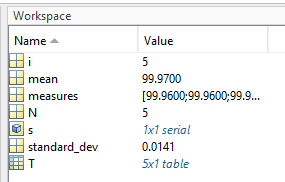
\includegraphics[width=.9\linewidth]{medias/test/repeatability/repeatability_results_0.png}
  \captionof{figure}{Test 1}
  \label{fig:test1}
\end{minipage}%
\begin{minipage}{.5\textwidth} % 40% della larghezza del testo
  \centering
  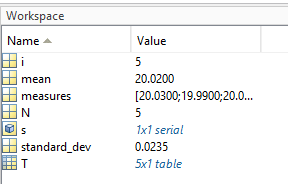
\includegraphics[width=.9\linewidth]{medias/test/repeatability/repeatability_results_1.png}
  \captionof{figure}{Test 2}
  \label{fig:test2}
\end{minipage}
\end{figure}

\noindent In the repeatability test, the instrument is first zeroed, then the load is placed on the plate and the indication is recorded once stabilized. Then the load is removed and the zero indication is checked and zeroed if necessary. Then the load is replaced and so on. For a scale with multiple fields / divisions, a test weight below the first range should be sufficient.

\clearpage

\subsection{MATLAB pseudocode}

\begin{verbatim}
clear the workspace and the screen
reset the serial devices

Set N to 5
Create a vector of N elements, initialized to zero
Ask the user to remove any object from the scale

create and open a serial connection with the scale

wait until the scale is ready

For each element of the vector
    Ask the user to place the object on the scale
    Receive a numeric value from the device
    Save the value in the vector and print it on the screen
    Ask the user to remove the object from the scale
End for

Close and delete the serial connection

Compute the mean and the standard deviation of the original vector
\end{verbatim}
\clearpage

\section{Eccentricity}

Eccentricity tests are performed on weighing instruments to measure how the position of the load affects the accuracy and repeatability of the readings. The principle of the test is to compare the indications of the instrument when the same load is applied at different locations on the load receptor. The locations are chosen according to the shape and the number of support points of the load receptor, following the standards OIML R76 and EN 45501. The test load should be at least one third of the maximum capacity of the instrument, and preferably a single load, to ensure the consistency of the center of gravity.\\
\begin{figure}[h]
    \centering
    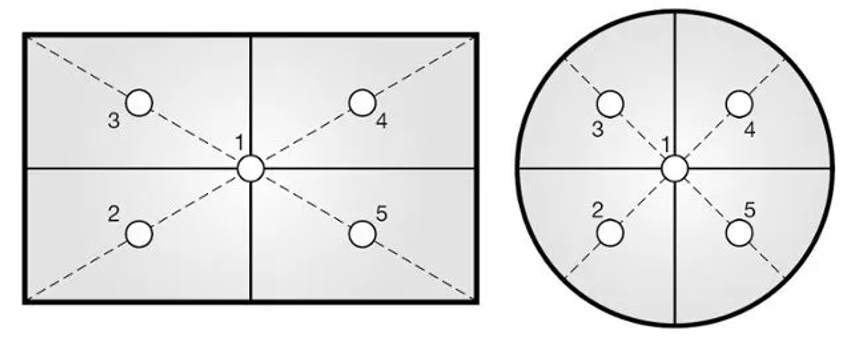
\includegraphics[width=0.8\textwidth]{medias/Scale_positions.png}
    \caption{Sample's positions}
    \label{fig:enter-label}
\end{figure}
\\
The test procedure consists of placing the test load at the center of the load receptor and recording the indication. Then, the load is moved to four other locations, usually at the corners or the edges of the load receptor, and the indications are recorded again. The load is then returned to the center and the indication is checked for any drift. The zero of the instrument may be verified and adjusted between each location, if needed. Alternatively, the instrument may be tared when the load is at the center, to make the differences between locations more visible. 
\clearpage

%inserire immagine 'eccentricity' e descrizione in forma tabellare 
\begin{figure}[h]
    \centering
    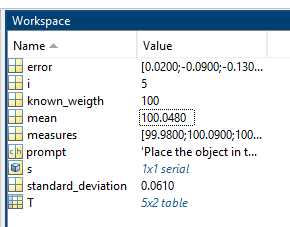
\includegraphics[width=0.5\textwidth]{medias/test/post/eccentricity.png}
    \caption{Workspace}
    \label{fig:enter-label}
\end{figure}

\noindent The test is considered passed if the differences between the indications at different locations are within the permissible errors specified by the standards or the manufacturer. The differences are also used to calculate the eccentricity error, which is the maximum deviation of the indication from the arithmetic mean of all indications. The eccentricity error is an important parameter to evaluate the performance and the quality of the weighing instrument.


\subsection{MATLAB pseudocode}

\begin{verbatim}
clear the workspace and the screen
reset the serial devices

Set N to 5
Create a vector of N elements, initialized to zero
Ask the user to remove any object from the scale

create and open a serial connection with the scale

wait until the scale is ready

For each position of the scale
    Ask the user to place the object on the scale
    Receive a numeric value from the device
    Save the value in the vector and print it on the screen
    Ask the user to remove the object from the scale
End for

Close and delete the serial connection

Compute the mean and the standard deviation of the original vector

Save the data in a table with two columns: measured weight and error
\end{verbatim}

\section{Hysteresis}

Hysteresis refers to the difference in a system’s output when a specific input is approached from increasing and decreasing directions. In weighing tests, it’s crucial not to overshoot or undershoot the load to accurately identify hysteresis. The instrument should be calibrated with increasing and decreasing points, approaching each test point with increasing or decreasing weight respectively.
\\
Multiple points throughout the instrument’s measurement range are used to reveal any linearity issues, which means the instrument does not measure equally accurate throughout its range. Even if the zero and full span are correct, there may be errors in the middle of the range, referred to as linearity errors, or non-linearity.
\\
The purpose of a weighing test is to test the calibrated accuracy of the weighing instrument across its entire range, in several steps, with increasing and decreasing weight. Typically, 5 to 10 different loads (test points) are used, and each range must be calibrated separately in multi-range instruments.

\subsection{MATLAB pseudocode}

\begin{verbatim}
clear the workspace and the screen
reset the serial devices

Set N to 5
Create a vector of 2*N elements, initialized to zero
Ask the user to remove any object from the scale

create and open a serial connection with the scale

wait until the scale is ready

For each measurement, up to N
    ask the user to enter the known weight (ascending order)
    Receive a numeric value from the device
    Save the value in the vector and print it on the screen
    Ask the user to remove the object from the scale
End for

For each measurement, for N+1 up to 2*N
    ask the user to enter the known weight (descending order)
    Receive a numeric value from the device
    Save the value in the vector and print it on the screen
    Ask the user to remove the object from the scale
End for

Close and delete the serial connection

plot the data
\end{verbatim}

\begin{quote}
\textbf{Note:} Try not to keep the scale turned on for a very long time, since it may lose precision due to the heating of the components.
\end{quote}